\chapter{Arquitectura general}
\section{Visión general}
ASTRA CLOUD se organiza en servicios de negocio, almacenamiento operacional y analítica. Las APIs se ejecutan como contenedores; PostgreSQL, MySQL y MongoDB almacenan la información de sus dominios. La Figura~\ref{fig:arquitectura_general} resume la arquitectura definida para integrar los componentes en AWS.
\begin{figure}[H]\centering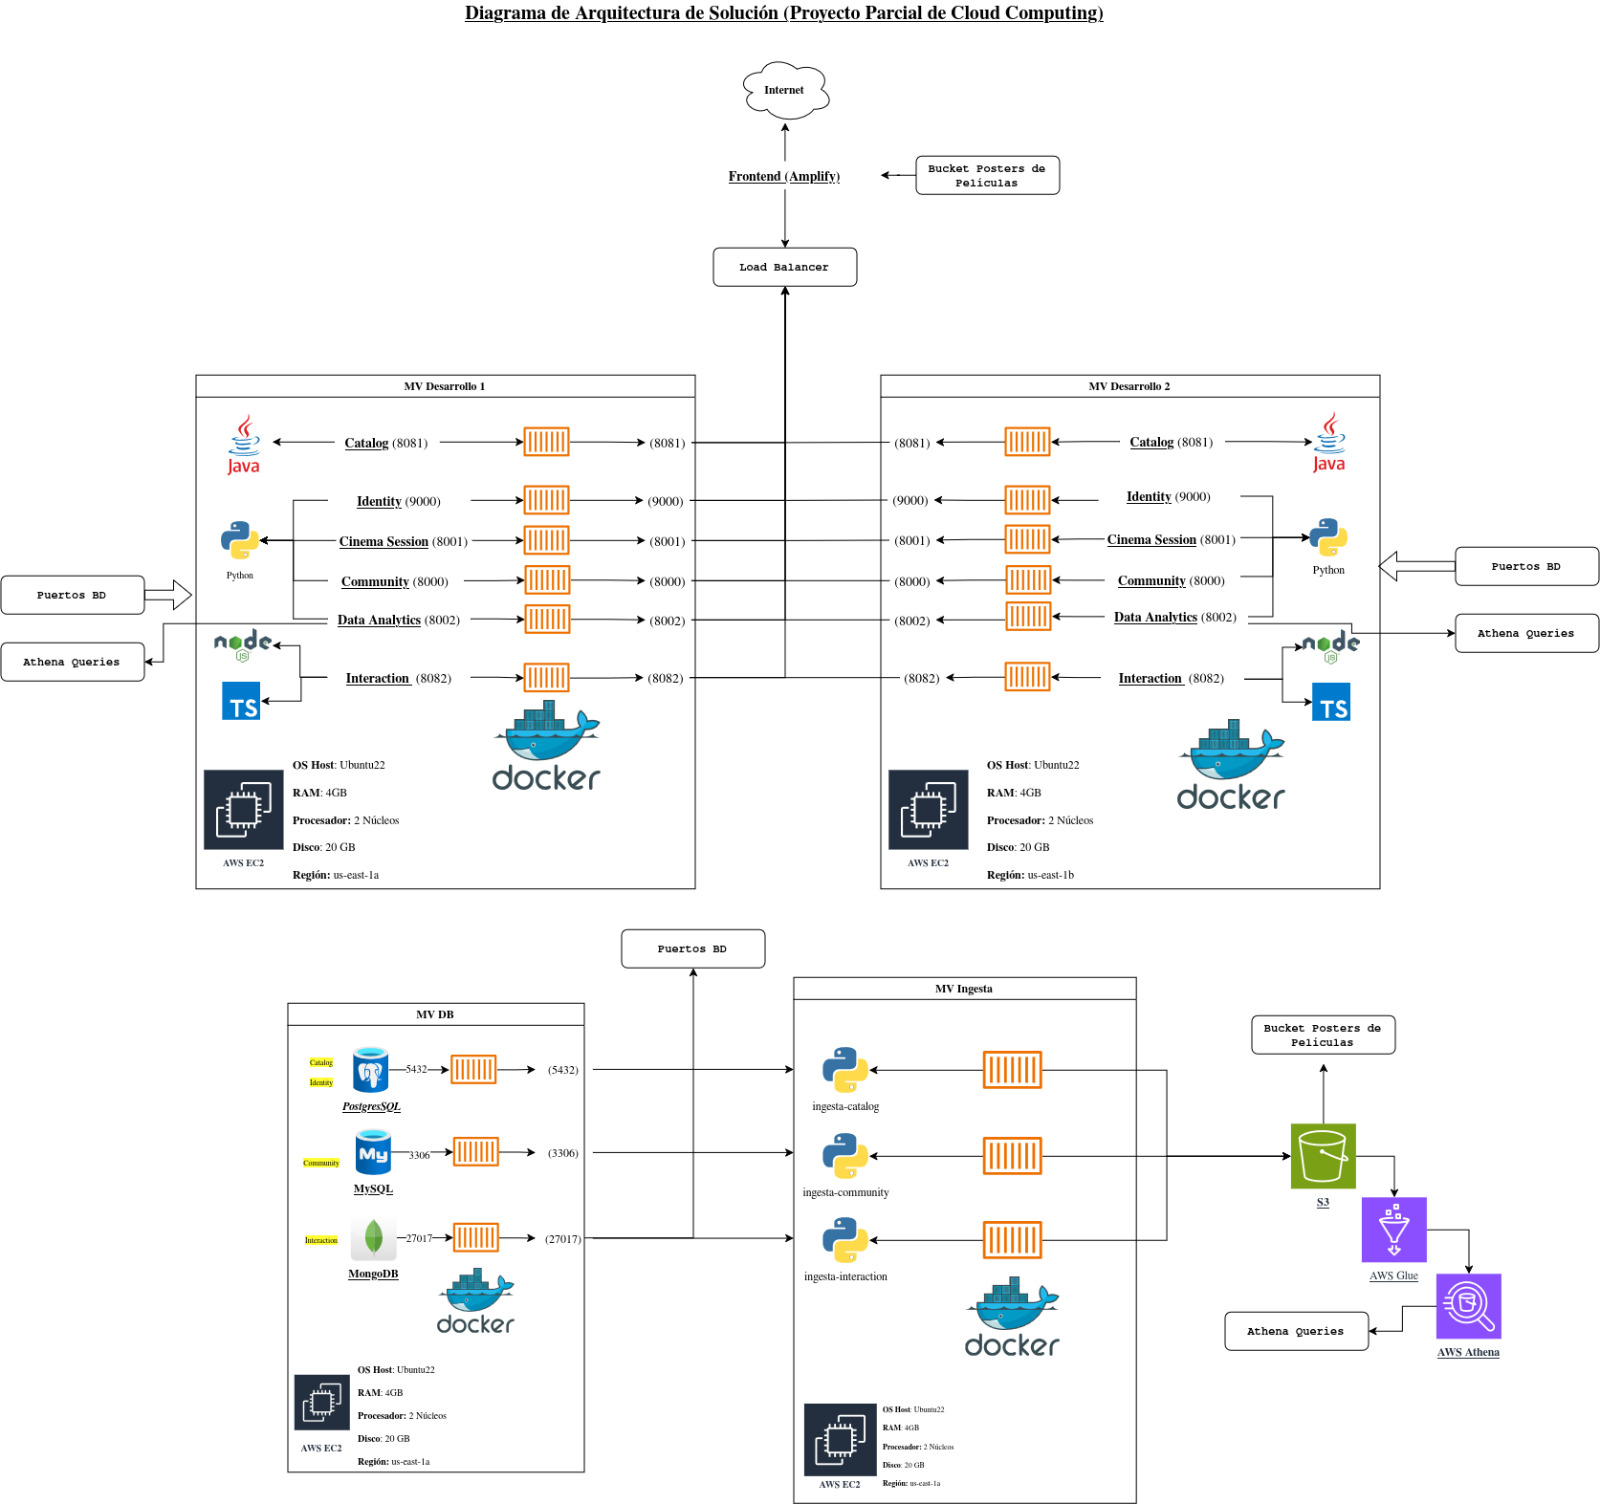
\includegraphics[width=.92\textwidth]{figures/arquitectura-general.jpeg}\caption{Arquitectura general de ASTRA CLOUD}\label{fig:arquitectura_general}\end{figure}
\section{Ruta de acceso}
Para el despliegue se definió la ruta cliente $\rightarrow$ API Gateway $\rightarrow$ VPC Link $\rightarrow$ ALB interno $\rightarrow$ listener por puerto $\rightarrow$ grupo destino $\rightarrow$ EC2 $\rightarrow$ contenedor. Esta separación centraliza el acceso a las APIs sin exponer directamente el balanceador.

